\section{Exercises}

%__________________
\subsection{Normal distribution}

% 1

\eoce{\qt{Area under the curve, I} What percent of a standard normal distribution $N(\mu=0, \sigma=1)$ is found in each region? Be sure to draw a graph. \vspace{-3mm}
\begin{multicols}{4}
\begin{parts}
\item $Z < -1.35$
\item $Z > 1.48$
\item $-0.4 < Z < 1.5$
\item $|Z| > 2$
\end{parts}
\end{multicols}
}{}

% 2

\eoce{\qt{Area under the curve, II} What percent of a standard normal distribution $N(\mu=0, \sigma=1)$ is found in each region? Be sure to draw a graph. \vspace{-3mm}
\begin{multicols}{4}
\begin{parts}
\item $Z > -1.13$
\item $Z < 0.18$
\item $Z > 8$
\item $|Z| < 0.5$
\end{parts}
\end{multicols}
}{}

% 3

\eoce{\qt{GRE scores, Part I\label{GRE}} Sophia who took the Graduate Record Examination (GRE) scored 160 on the Verbal Reasoning section and 157 on the Quantitative Reasoning section. The mean score for Verbal Reasoning section for all test takers was 151 with a standard deviation of 7, and the mean score for the Quantitative Reasoning was 153 with a standard deviation of 7.67. Suppose that both distributions are nearly normal. 
\begin{parts}
\item Write down the short-hand for these two normal distributions.
\item What is  Sophia's Z-score on the Verbal Reasoning section? On the Quantitative Reasoning section? Draw a standard normal distribution curve and mark these two Z-scores.
\item What do these Z-scores tell you?
\item Relative to others, which section did she do better on?
\item Find her percentile scores for the two exams.
\item What percent of the test takers did better than her on the Verbal Reasoning section? On the Quantitative Reasoning section?
\item Explain why simply comparing her raw scores from the two sections would lead to the incorrect conclusion that she did better on the Quantitative Reasoning section.
\item If the distributions of the scores on these exams are not nearly normal, would your answers to parts (b) - (f) change? Explain your reasoning.
\end{parts}
}{}

% 4

\eoce{\qt{Triathlon times, Part I} \label{triathlon} In triathlons, it is common for racers to be placed into age and gender groups. Friends Leo and Mary both completed the Hermosa Beach Triathlon, where Leo competed in the \textit{Men, Ages 30 - 34} group while Mary competed in the \textit{Women, Ages 25 - 29} group. Leo completed the race in 1:22:28 (4948 seconds), while Mary completed the race in 1:31:53 (5513 seconds). Obviously Leo finished faster, but they are curious about how they did within their respective groups. Can you help them?
Here is some information on the performance of their groups:
\begin{itemize}
\setlength{\itemsep}{0mm}
\item The finishing times of the \textit{Men, Ages 30 - 34} group has a mean of 4313 seconds with a standard deviation of 583 seconds.
\item The finishing times of the \textit{Women, Ages 25 - 29} group has a mean of 5261 seconds with a standard deviation of 807 seconds.
\item The distributions of finishing times for both groups are approximately Normal.
\end{itemize}
Remember: a better performance corresponds to a faster finish.
\begin{parts}
\item Write down the short-hand for these two normal distributions.
\item What are the Z-scores for Leo's and Mary's finishing times? What do these Z-scores tell you?
\item Did Leo or Mary rank better in their respective groups? Explain your reasoning.
\item What percent of the triathletes did Leo finish faster than in his group?
\item What percent of the triathletes did Mary finish faster than in her group?
\item If the distributions of finishing times are not nearly normal, would your answers to parts (b)~-~(e) change? Explain your reasoning.
\end{parts}
}{}

% 5

\eoce{\qt{GRE scores, Part II} In Exercise~\ref{GRE} we saw two distributions for GRE scores: $N(\mu=151, \sigma=7)$ for the verbal part of the exam and $N(\mu=153, \sigma=7.67)$ for the quantitative part. Use this information to compute each of the following:
\begin{parts}
\item The score of a student who scored in the $80^{th}$ percentile on the Quantitative Reasoning section.
\item The score of a student who scored worse than 70\% of the test takers in the Verbal Reasoning section.
\end{parts}
}{}

% 6

\eoce{\qt{Triathlon times, Part II} In Exercise~\ref{triathlon} we saw two distributions for triathlon times: $N(\mu=4313, \sigma=583)$ for \emph{Men, Ages 30 - 34} and $N(\mu=5261, \sigma=807)$ for the \emph{Women, Ages 25 - 29} group. Times are listed in seconds. Use this information to compute each of the following:
\begin{parts}
\item The cutoff time for the fastest 5\% of athletes in the men's group, i.e. those who took the shortest 5\% of time to finish. 
\item The cutoff time for the slowest 10\% of athletes in the women's group. 
\end{parts}
}{}

% 7

\eoce{\qt{LA weather, Part I} \label{tempLA} The average daily high temperature in June in LA is 77\degree F with a standard deviation of 5\degree F. Suppose that the temperatures in June closely follow a normal distribution. 
\begin{parts}
\item What is the probability of observing an 83\degree F temperature or higher in LA during a randomly chosen day in June?
\item How cold are the coldest 10\% of the days during June in LA?
\end{parts}
}{}

% 8

\eoce{\qt{Portfolio returns} The Capital Asset Pricing Model is a financial model that assumes returns on a portfolio are normally distributed. Suppose a portfolio has an average annual return of 14.7\% (i.e. an average gain of 14.7\%) with a standard deviation of 33\%. A return of 0\% means the value of the portfolio doesn't change, a negative return means that the portfolio loses money, and a positive return means that the portfolio gains money.
\begin{parts}
\item What percent of years does this portfolio lose money, i.e. have a return less than 0\%?
\item What is the cutoff for the highest 15\% of annual returns with this portfolio?
\end{parts}
}{}

% 9

\eoce{\qt{LA weather, Part II} Exercise~\ref{tempLA} states that average daily high temperature in June in LA is 77\degree F with a standard deviation of 5\degree F, and it can be assumed that they to follow a normal distribution. We use the following equation to convert \degree F (Fahrenheit) to \degree C (Celsius):
\[ C = (F - 32) \times \frac{5}{9}. \]
\begin{parts}
\item Write the probability model for the distribution of temperature in \degree C in June in LA.
\item What is the probability of observing a 28\degree C (which roughly corresponds to 83\degree F) temperature or higher in June in LA? Calculate using the \degree C model from part (a).
\item Did you get the same answer or different answers in part (b) of this question and part (a) of Exercise~\ref{tempLA}? Are you surprised? Explain.
\item Estimate the IQR of the the temperatures (in \degree C) in June in LA?
\end{parts}
}{}

% 10

\eoce{\qt{Heights of 10 year olds} Heights of 10 year olds, regardless of gender, closely follow a normal distribution with mean 55 inches and standard deviation 6 inches.
\begin{parts}
\item What is the probability that a randomly chosen 10 year old is shorter than 48 inches?
\item What is the probability that a randomly chosen 10 year old is between 60 and 65 inches?
\item If the tallest 10\% of the class is considered ``very tall", what is the height cutoff for ``very tall"?
\item The height requirement for \textit{Batman the Ride} at Six Flags Magic Mountain is 54 inches. What percent of 10 year olds cannot go on this ride?
\end{parts}
}{}

% 11

\eoce{\qt{Auto insurance premiums} Suppose a newspaper article states that the distribution of auto insurance premiums for residents of California is approximately normal with a mean of \$1,650. The article also states that 25\% of California residents pay more than \$1,800. 
\begin{parts}
\item What is the Z-score that corresponds to the top 25\% (or the $75^{th}$ percentile) of the standard normal distribution?
\item What is the mean insurance cost? What is the cutoff for the 75th percentile?
\item Identify the standard deviation of insurance premiums in LA.
\end{parts}
}{}

% 12

\eoce{\qt{Speeding on the I-5, Part I} \label{i5} The distribution of passenger vehicle speeds traveling on the Interstate 5 Freeway (I-5) in California is nearly normal with a mean of 72.6 miles/hour and a standard deviation of 4.78 miles/hour.\footfullcite{Johnson+Murray:2010}
\begin{parts}
\item What percent of passenger vehicles travel slower than 80 miles/hour?
\item What percent of passenger vehicles travel between 60 and 80 miles/hour?
\item How fast do the fastest 5\% of passenger vehicles travel?
\item The speed limit on this stretch of the I-5 is 70 miles/hour. Approximate what percentage of the passenger vehicles travel above the speed limit on this stretch of the I-5.
\end{parts}
}{}

% 13

\eoce{\qt{Overweight baggage, Part I} Suppose weights of the checked baggage of airline passengers follow a nearly normal distribution with mean 45 pounds and standard deviation 3.2 pounds. Most airlines charge a fee for baggage that weigh in excess of 50 pounds. Determine what percent of airline passengers incur this fee.
}{}

% 14

\eoce{\qt{Find the SD} Find the standard deviation of the distribution in the following situations.
\begin{parts}
\item  MENSA is an organization whose members have IQs in the top 2\% of the population. IQs are normally distributed with mean 100, and the minimum IQ score required for admission to MENSA is 132.
\item Cholesterol levels for women aged 20 to 34 follow an approximately normal distribution with mean 185 milligrams per deciliter (mg/dl). Women with cholesterol levels above 220 mg/dl are considered to have high cholesterol and about 18.5\% of women fall into this category.
\end{parts}
}{}

% 15

\eoce{\qt{Buying books on Ebay} The textbook you need to buy for your chemistry class is expensive at the college bookstore, so you consider buying it on Ebay instead. A look at past auctions suggest that the prices of that chemistry textbook have an approximately normal distribution with mean \$89 and standard deviation \$15. 
\begin{parts}

\item What is the probability that a randomly selected auction for this book closes at more than \$100?

\item Ebay allows you to set your maximum bid price so that if someone outbids you on an auction you can automatically outbid them, up to the maximum bid price you set. If you are only bidding on one auction, what are the advantages and disadvantages of setting a bid price too high or too low? What if you are bidding on multiple auctions?

\item If you watched 10 auctions, roughly what percentile might you use for a maximum bid cutoff to be somewhat sure that you will win one of these ten auctions? Is it possible to find a cutoff point that will ensure that you win an auction?

\item If you are willing to track up to ten auctions closely, about what price might you use as your maximum bid price if you want to be somewhat sure that you will buy one of these ten books?

\end{parts}
}{}

\textA{\pagebreak}

% 16

\eoce{\qt{SAT scores} SAT scores (out of 2400) are distributed normally with a mean of 1500 and a standard deviation of 300. Suppose a school council awards a certificate of excellence to all students who score at least 1900 on the SAT, and suppose we pick one of the recognized students at random. What is the probability this student's score will be at least 2100? (The material covered in Section~\ref{conditionalProbabilitySection} would be useful for this question.)
}{}

% 17

\eoce{\qt{Scores on stats final, Part I} \label{statsScores} Below are final exam scores of 20 Introductory Statistics students. 
\[ \stackrel{1}{57}, \stackrel{2}{66}, \stackrel{3}{69}, \stackrel{4}{71}, \stackrel{5}{72}, \stackrel{6}{73}, \stackrel{7}{74}, \stackrel{8}{77}, \stackrel{9}{78}, \stackrel{10}{78}, \stackrel{11}{79}, \stackrel{12}{79}, \stackrel{13}{81}, \stackrel{14}{81}, \stackrel{15}{82}, \stackrel{16}{83}, \stackrel{17}{83}, \stackrel{18}{88}, \stackrel{19}{89}, \stackrel{20}{94} \]
The mean score is 77.7 points. with a standard deviation of 8.44 points. Use this information to determine if the scores approximately follow the 68-95-99.7\% Rule.
}{}

% 18

\eoce{\qt{Heights of female college students, Part I} \label{collegeFemHeights} Below are heights of 25 female college students.
\[ \stackrel{1}{54}, \stackrel{2}{55}, \stackrel{3}{56}, \stackrel{4}{56}, \stackrel{5}{57}, \stackrel{6}{58}, \stackrel{7}{58}, \stackrel{8}{59}, \stackrel{9}{60}, \stackrel{10}{60}, \stackrel{11}{60}, \stackrel{12}{61}, \stackrel{13}{61}, \stackrel{14}{62}, \stackrel{15}{62}, \stackrel{16}{63}, \stackrel{17}{63}, \stackrel{18}{63}, \stackrel{19}{64}, \stackrel{20}{65}, \stackrel{21}{65}, \stackrel{22}{67}, \stackrel{23}{67}, \stackrel{24}{69}, \stackrel{25}{73} \]
The mean height is 61.52 inches with a standard deviation of 4.58 inches. Use this information to determine if the heights approximately follow the 68-95-99.7\% Rule.
}{}

% 19

\eoce{\qt{Scores on stats final, Part II} Exercise~\ref{statsScores} lists the final exam scores of 20 Introductory Statistics students. Do these data appear to follow a normal distribution? Explain your reasoning using the graphs provided below.
\begin{center}
\includegraphics[width=0.46\textwidth]{ch_distributions/figures/eoce/scores/scores_hist}\ \ \ \ 
\includegraphics[width= 0.46\textwidth]{ch_distributions/figures/eoce/scores/scores_qq}
\end{center}
}{}

% 20

\eoce{\qt{Heights of female college students, Part II} Exercise~\ref{collegeFemHeights} lists the heights of 25 female college students. Do these data appear to follow a normal distribution? Explain your reasoning using the graphs provided below.
\begin{center}
\includegraphics[width= 0.46\textwidth]{ch_distributions/figures/eoce/heightsFcoll/heightsFcoll_hist}\ \ \ \ 
\includegraphics[width= 0.46\textwidth]{ch_distributions/figures/eoce/heightsFcoll/heightsFcoll_qq}
\end{center}
}{}

\textA{\pagebreak}

% 21

\eoce{\qt{Lemonade at The Cafe} Drink pitchers at The Cafe are intended to hold about 64 ounces of lemonade and glasses hold about 12 ounces. However, when the pitchers are filled by a server, they do not always fill it with exactly 64 ounces. There is some variability. Similarly, when they pour out some of the lemonade, they do not pour exactly 12 ounces. The amount of lemonade in a pitcher is normally distributed with mean 64 ounces and standard deviation 1.732 ounces. The amount of lemonade in a glass is normally distributed with mean 12 ounces and standard deviation 1 ounce. 
\begin{parts}
\item How much lemonade would you expect to be left in a pitcher after pouring one glass of lemonade? 
\item What is the standard deviation of the amount left in a pitcher after pouring one glass of lemonade? 
\item What is the probability that more than 50 ounces of lemonade is left in a pitcher after pouring one glass of lemonade?
\end{parts}
}{}

% 22

\eoce{\qt{Spray paint, Part I} \label{sprayPaint} Suppose the area that can be painted using a single can of spray paint is slightly variable and follows a nearly normal distribution with a mean of 25 square feet and a standard deviation of 3 square feet. Suppose also that you buy three cans of spray paint.
\begin{parts}
\item How much area would you expect to cover with these three cans of spray paint?
\item What is the standard deviation of the area you expect to cover with these three cans of spray paint?
\item The area you wanted to cover is 80 square feet. What is the probability that you will be able to cover this entire area with these three cans of spray paint?
\end{parts}
}{}

% 23

\eoce{\qt{GRE scores, Part III} In Exercise~\ref{GRE} we saw two distributions for GRE scores: $N(\mu=151, \sigma=7)$ for the verbal part of the exam and $N(\mu=153, \sigma=7.67)$ for the quantitative part. Suppose performance on these two sections is independent. Use this information to compute each of the following:
\begin{parts}
\item The probability of a combined (verbal + quantitative) score above 320. 
\item The score of a student who scored better than 90\% of the test takers overall.
\end{parts}
}{}

% 24
\eoce{\qt{Betting on dinner, Part I} \label{dinnerBet} Suppose a restaurant is running a promotion where prices of menu items are determined randomly following some underlying distribution. This means that if you're lucky you can get a basket of fries for \$3, or if you're not so lucky you might end up having to pay \$10 for the same menu item. The price of basket of fries is drawn from a normal distribution with mean 6 and standard deviation of 2. The price of a fountain drink is drawn from a normal distribution with mean 3 and standard deviation of 1. What is the probability that you pay more than \$10 for a dinner consisting of a basket of fries and a fountain drink?}
{}

\textA{\newpage}

%__________________
\subsection{Sampling distribution of a sample mean}

% 25

\eoce{\qt{Ages of pennies, Part I} \label{penniesAges} The histogram below shows the distribution of ages of pennies at a bank. 

\noindent\begin{minipage}[c]{0.54\textwidth}
\begin{parts}
\item Describe the distribution.
\item Sampling distributions for means from simple random samples of 5, 30, and 100 pennies is shown in the histograms below. Describe the shapes of these distributions and comment on whether they look like what you would expect to see based on the Central Limit Theorem.
\end{parts}
\end{minipage}
\begin{minipage}[c]{0.44\textwidth}
\begin{center}
\includegraphics[width=\textwidth]{ch_distributions/figures/eoce/penniesAges/penniesAges_pop} 
\end{center}
\end{minipage}\vspace{-1mm}
\begin{center}
\includegraphics[width=0.325\textwidth]{ch_distributions/figures/eoce/penniesAges/penniesAges_n5} 
\includegraphics[width= 0.325\textwidth]{ch_distributions/figures/eoce/penniesAges/penniesAges_n30} 
\includegraphics[width= 0.325\textwidth]{ch_distributions/figures/eoce/penniesAges/penniesAges_n100} 
\end{center}
}{}

% 26

\eoce{\qt{Ages of pennies, Part II} The mean age of the pennies from Exercise~\ref{penniesAges} is 10.44 years with a standard deviation of 9.2 years. Using the Central Limit Theorem, calculate the means and standard deviations of the distribution of the mean from random samples of size 5, 30, and 100. Comment on whether the sampling distributions shown in Exercise~\ref{penniesAges} agree with the values you compute.
}{}

% 27

\eoce{\qt{Housing prices, Part I} \label{Topanga} A housing survey was conducted to determine the price of a typical home in Topanga, CA. The mean price of a house was roughly \$1.3 million with a standard deviation of \$300,000. There were no houses listed below \$600,000 but a few houses above \$3 million.
\begin{parts}
\item Is the distribution of housing prices in Topanga symmetric, right skewed, or left skewed? \textit{Hint:} Sketch the distribution.
\item Would you expect most houses in Topanga to cost more or less than \$1.3 million?
\item Can we estimate the probability that a randomly chosen house in Topanga costs more than \$1.4 million using the normal distribution?
\item What is the probability that the mean of 60 randomly chosen houses in Topanga is more than \$1.4 million?
\item How would doubling the sample size affect the standard deviation of the mean?
\end{parts}
}{}

% 28

\eoce{\qt{Stats final scores} Each year about 1500 students take the introductory statistics course at a large university. This year scores on the final exam are distributed with a median of 74 points, a mean of 70 points, and a standard deviation of 10 points. There are no students who scored above 100 (the maximum score attainable on the final) but a few students scored below 20 points.
\begin{parts}
\item Is the distribution of scores on this final exam symmetric, right skewed, or left skewed?
\item Would you expect most students to have scored above or below 70 points?
\item Can we calculate the probability that a randomly chosen student scored above 75 using the normal distribution?
\item What is the probability that the average score for a random sample of 40 students is above 75?
\item How would cutting the sample size in half affect the standard deviation of the mean?
\end{parts}
}{}

% 29

\eoce{\qt{Identify distributions, Part I} Four plots are presented below. The plot at the top is a distribution for a population. The mean is 10 and the standard deviation is 3. Also shown below is a distribution of (1) a single random sample of 100 values from this population, (2) a distribution of 100 sample means from random samples with size 5, and (3) a distribution of 100 sample means from random samples with size 25. Determine which plot (A, B, or C) is which and explain your reasoning.
\begin{center}
\includegraphics[width=0.55\textwidth]{ch_distributions/figures/eoce/cltSimSYM/cltSimSYM_pop}
\end{center}
\begin{center}
\includegraphics[width=0.325\textwidth]{ch_distributions/figures/eoce/cltSimSYM/cltSimSYM_n5}
\includegraphics[width=0.325\textwidth]{ch_distributions/figures/eoce/cltSimSYM/cltSimSYM_samp}
\includegraphics[width=0.325\textwidth]{ch_distributions/figures/eoce/cltSimSYM/cltSimSYM_n25}
\end{center}
}{}

% 30

\eoce{\qt{Identify distributions, Part II} Four plots are presented below. The plot at the top is a distribution for a population. The mean is 60 and the standard deviation is 18. Also shown below is a distribution of (1) a single random sample of 500 values from this population, (2) a distribution of 500 sample means from random samples of each size 18, and (3) a distribution of 500 sample means from random samples of each size 81. Determine which plot (A, B, or C) is which and explain your reasoning.
\begin{center}
\includegraphics[width=0.55\textwidth]{ch_distributions/figures/eoce/cltSimLS/cltSimLS_pop}
\end{center}
\begin{center}
\includegraphics[width=0.325\textwidth]{ch_distributions/figures/eoce/cltSimLS/cltSimLS_n81}
\includegraphics[width=0.325\textwidth]{ch_distributions/figures/eoce/cltSimLS/cltSimLS_samp}
\includegraphics[width=0.325\textwidth]{ch_distributions/figures/eoce/cltSimLS/cltSimLS_n18}
\end{center}
}{} 

\textA{\pagebreak}

% 31

\eoce{\qt{Weights of pennies} The distribution of weights of United States pennies is approximately normal with a mean of 2.5 grams and a standard deviation of 0.03 grams.
\begin{parts}
\item What is the probability that a randomly chosen penny weighs less than 2.4 grams?
\item Describe the sampling distribution of the mean weight of 10 randomly chosen pennies.
\item What is the probability that the mean weight of 10 pennies is less than 2.4 grams?
\item Sketch the two distributions (population and sampling) on the same scale.
\item Could you estimate the probabilities from (a) and (c) if the weights of pennies had a skewed distribution?
\end{parts}
}{}

% 32

\eoce{\qt{CFLs} A manufacturer of compact fluorescent light bulbs advertises that the distribution of the lifespans of these light bulbs is nearly normal with a mean of 9,000 hours and a standard deviation of 1,000 hours.
\begin{parts}
\item What is the probability that a randomly chosen light bulb lasts more than 10,500 hours?
\item Describe the distribution of the mean lifespan of 15 light bulbs. 
\item What is the probability that the mean lifespan of 15 randomly chosen light bulbs is more than 10,500 hours?
\item Sketch the two distributions (population and sampling) on the same scale.
\item Could you estimate the probabilities from parts~(a) and~(c) if the lifespans of light bulbs had a skewed distribution?
\end{parts}
}{}

% 33

\eoce{\qt{Songs on an  iPod} Suppose an iPod has 3,000 songs. The histogram below shows the distribution of the lengths of these songs. We also know that, for this iPod, the mean length is 3.45 minutes and the standard deviation is 1.63 minutes.
\begin{center}
\includegraphics[width=0.5\textwidth]{ch_distributions/figures/eoce/ipod/ipod_popdist}
\end{center}
\begin{parts}
\item Calculate the probability that a randomly selected song lasts more than 5 minutes.
\item You are about to go for an hour run and you make a random playlist of 15 songs. What is the probability that your playlist lasts for the entire duration of your run? \textit{Hint:} If you want the playlist to last 60 minutes, what should be the minimum average length of a song?
\item You are about to take a trip to visit your parents and the drive is 6 hours. You make a random playlist of 100 songs. What is the probability that your playlist lasts the entire drive?
\end{parts}
}{}

% 34

\eoce{\qt{Spray paint, Part II} As described in Exercise~\ref{sprayPaint}, the area that can be painted using a single can of spray paint is slightly variable and follows a nearly normal distribution with a mean of 25 square feet and a standard deviation of 3 square feet. 
\begin{parts}
\item What is the probability that the area covered by a can of spray paint is more than 27 square feet?
\item Suppose you want to spray paint an area of 540 square feet using 20 cans of spray paint. On average, how many square feet must each can be able to cover to spray paint all 540 square feet?
\item What is the probability that you can cover a 540 square feet area using 20 cans of spray paint?
\item If the area covered by a can of spray paint had a slightly skewed distribution, could you still calculate the probabilities in parts~(a) and~(c) using the normal distribution?
\end{parts}
}{}

% 35

\eoce{\qt{Wireless routers} John is shopping for wireless routers and is overwhelmed by the number of available options. In order to get a feel for the average price, he takes a random sample of 75 routers and finds that the average price for this sample is \$75 and the standard deviation is \$25. 
\begin{parts}
\item Based on this information, how much variability should he expect to see in the mean prices of repeated samples, each containing 75 randomly selected wireless routers?
\item A consumer website claims that the average price of routers is \$80. Is a true average of \$80 consistent with John's sample?
\end{parts}
}{}

%36

\eoce{\qt{Chocolate chip cookies} Students are asked to count the number of chocolate chips in 22 cookies for a class activity. The packaging for these cookies claims that there are an average of 20 chocolate chips per cookie with a standard deviation of 4.37 chocolate chips.
\begin{parts}
\item Based on this information, about how much variability should they expect to see in the mean number of chocolate chips in random samples of 22 chocolate chip cookies?
\item What is the probability that a random sample of 22 cookies will have an average less than 14.77 chocolate chips if the companies claim on the packaging is true?
\item Assume the students got 14.77 as the average in their sample of 22 cookies.  Do you have have confidence or not in the company's claim that the true average is 20?  Explain your reasoning.
\end{parts}
}{}

% 37

\eoce{\qt{Overweight baggage, Part II} Suppose weights of the checked baggage of airline passengers follow a nearly normal distribution with mean 45 pounds and standard deviation 3.2 pounds. What is the probability that the \emph{total} weight of 10 bags is greater than 460 lbs?
}{}

% 38

\eoce{\qt{Betting on dinner, Part II} Exercise~\ref{dinnerBet} introduces a promotion at a restaurant where prices of menu items are determined randomly following some underlying distribution. We are told that the price of basket of fries is drawn from a normal distribution with mean 6 and standard deviation of 2. You want to get 5 baskets of fries but you only have \$28 in your pocket. What is the probability that you would have enough money to pay for all five baskets of fries?}
{}

%__________________
\subsection{Geometric distribution}

% 39

\eoce{\qtq{Is it Bernoulli} Determine if each trial can be considered an independent Bernouilli trial for the following situations.
\begin{parts}
\item Cards dealt in a hand of poker.
\item Outcome of each roll of a die.
\end{parts}
}{}

% 40

\eoce{\qt{With and without replacement} In the following situations assume that half of the specified population is male and the other half is female.
\begin{parts}
\item Suppose you're sampling from a room with 10 people. What is the probability of sampling two females in a row when sampling with replacement? What is the probability when sampling without replacement?
\item Now suppose you're sampling from a stadium with 10,000 people. What is the probability of sampling two females in a row when sampling with replacement? What is the probability when sampling without replacement?
\item We often treat individuals who are sampled from a large population as independent. Using your findings from parts~(a) and~(b), explain whether or not this assumption is reasonable.
\end{parts}
}{}

\textA{\pagebreak}

% 41

\eoce{\qt{Married women} \label{marriedWomen} The 2010 American Community Survey estimates that 47.1\% of women ages 15 years and over are married.\footfullcite{marWomenACS}
\begin{parts}
\item We randomly select three women between these ages. What is the probability that the third woman selected is the only one who is married?
\item What is the probability that all three randomly selected women are married?
\item On average, how many women would you expect to sample before selecting a married woman? What is the standard deviation?
\item If the proportion of married women was actually 30\%, how many women would you expect to sample before selecting a married woman? What is the standard deviation?
\item Based on your answers to parts (c) and (d), how does decreasing the probability of an event affect the mean and standard deviation of the wait time until success?
\end{parts}
}{}

% 42

\eoce{\qt{Defective rate} \label{transistorLow} A machine that produces a special type of transistor (a component of computers) has a 2\% defective rate. The production is considered a random process where each transistor is independent of the others.
\begin{parts}
\item What is the probability that the $10^{th}$ transistor produced is the first with a defect?
\item What is the probability that the machine produces no defective transistors in a batch of 100?
\item On average, how many transistors would you expect to be produced before the first with a defect? What is the standard deviation?
\item Another machine that also produces transistors has a 5\% defective rate where each transistor is produced independent of the others. On average how many transistors would you expect to be produced with this machine before the first with a defect? What is the standard deviation?
\item Based on your answers to parts (c) and (d), how does increasing the probability of an event affect the mean and standard deviation of the wait time until success?
\end{parts}
}{}

% 43

\eoce{\qt{Eye color, Part I} \label{eyeColor} A husband and wife both have brown eyes but carry genes that make it possible for their children to have brown eyes (probability 0.75), blue eyes (0.125), or green eyes (0.125).
\begin{parts}
\item What is the probability the first blue-eyed child they have is their third child? Assume that the eye colors of the children are independent of each other.
\item On average, how many children would such a pair of parents have before having a blue-eyed child? What is the standard deviation of the number of children they would expect to have until the first blue-eyed child?
\end{parts}
}{}

% 44

\eoce{\qt{Speeding on the I-5, Part II} \label{i5Geom} Exercise~\ref{i5} states that the distribution of speeds of cars traveling on the Interstate 5 Freeway (I-5) in California is nearly normal with a mean of 72.6 miles/hour and a standard deviation of 4.78 miles/hour. The speed limit on this stretch of the I-5 is 70 miles/hour.
\begin{parts}
\item A highway patrol officer is hidden on the side of the freeway. What is the probability that 5~cars pass and none are speeding? Assume that the speeds of the cars are independent of each other.
\item On average, how many cars would the highway patrol officer expect to watch until the first car that is speeding? What is the standard deviation of the number of cars he would expect to watch?
\end{parts}
}{}

\textA{\pagebreak}

%__________________
\subsection{Binomial distribution}

% 45

\eoce{\qt{Underage drinking, Part II} We learned in Exercise~\ref{alcohol} that about 70\% of 18-20 year olds consumed alcoholic beverages in 2008. We now consider a random sample of fifty 18-20 year olds.
\begin{parts}
\item How many people would you expect to have consumed alcoholic beverages? And with what standard deviation?
\item Would you be surprised if there were 45 or more people who have consumed alcoholic beverages?
\item What is the probability that 45 or more people in this sample have consumed alcoholic beverages? How does this probability relate to your answer to part (b)?
\end{parts}
}{}

% 46

\eoce{\qt{Chickenpox, Part II} We learned in Exercise~\ref{chickenpox} that about 90\% of American adults had chickenpox before adulthood. We now consider a random sample of 120 American adults.
\begin{parts}
\item How many people in this sample would you expect to have had chickenpox in their childhood? And with what standard deviation?
\item Would you be surprised if there were 105 people who have had chickenpox in their childhood?
\item What is the probability that 105 or fewer people in this sample have had chickenpox in their childhood? How does this probability relate to your answer to part (b)?
\end{parts}
}{}

% 47

\eoce{\qt{University admissions} Suppose a university announced that it admitted 2,500 students for the following year's freshman class. However, the university has dorm room spots for only 1,786 freshman students. If there is a 70\% chance that an admitted student will decide to accept the offer and attend this university, what is the approximate probability that the university will not have enough dormitory room spots for the freshman class?
}{}

% 48

\eoce{\qt{Survey response rate} Pew Research reported in 2012 that the typical response rate to their surveys is only 9\%. If for a particular survey 15,000 households are contacted, what is the probability that at least 1,500 will agree to respond? \footfullcite{surveysPew}
}{}

% 49

\eoce{\qt{Game of dreidel} A dreidel is a four-sided spinning top with the Hebrew letters \textit{nun}, \textit{gimel}, \textit{hei}, and \textit{shin}, one on each side. Each side is equally likely to come up in a single spin of the dreidel. Suppose you spin a dreidel three times. Calculate the probability of getting

\noindent\begin{minipage}[c]{0.43\textwidth}
%\begin{multicols}{2}
\begin{parts}
\item at least one \textit{nun}? 
\item exactly 2 \textit{nun}s? 
\item exactly 1 \textit{hei}? 
\item at most 2 \textit{gimel}s? \vspace{3mm}
\end{parts}
%\end{multicols}
\end{minipage}%
\begin{minipage}[c]{0.27\textwidth}
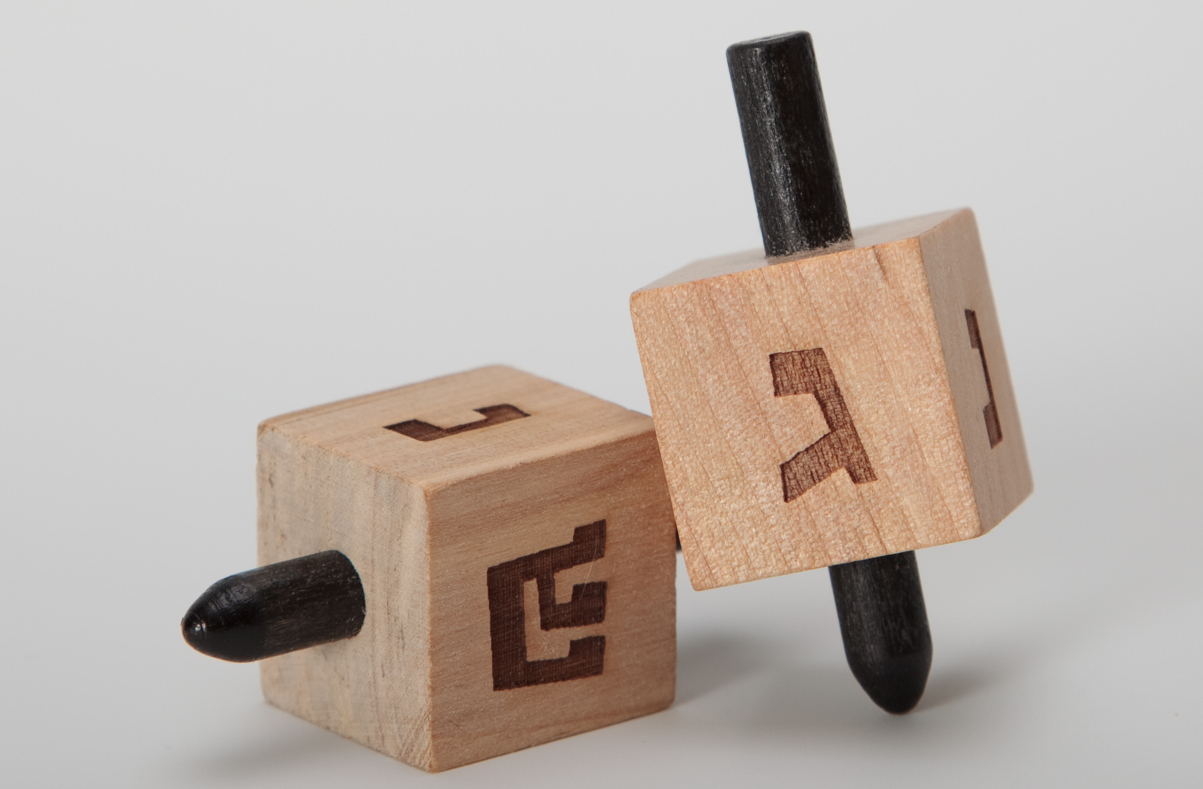
\includegraphics[width=0.9\textwidth]{ch_distributions/figures/eoce/images/dreidel_cropped}
\end{minipage}%
\begin{minipage}[c]{0.28\textwidth}%
{\footnotesize Photo by Staccabees, cropped \\
  (\oiRedirect{textbook-flickr_staccabees_dreidels}{http://flic.kr/p/7gLZTf}) \\
  \oiRedirect{textbook-CC_BY_2}{CC~BY~2.0~license}} \\[3mm] \
\end{minipage}
}{}

% 50

\eoce{\qt{Arachnophobia} A 2005 Gallup Poll found that that 7\% of teenagers (ages 13 to 17) suffer from arachnophobia and are extremely afraid of spiders. At a summer camp there are 10 teenagers sleeping in each tent. Assume that these 10 teenagers are independent of each other.\footfullcite{webpage:spiders}
\begin{parts}
\item Calculate the probability that at least one of them suffers from arachnophobia.
\item Calculate the probability that exactly 2 of them suffer from arachnophobia?
\item Calculate the probability that at most 1 of them suffers from arachnophobia? 
\item If the camp counselor wants to make sure no more than 1 teenager in each tent is afraid of spiders, does it seem reasonable for him to randomly assign teenagers to tents?
\end{parts}
}{}

% 51

\eoce{\qt{Eye color, Part II} Exercise~\ref{eyeColor} introduces a husband and wife with brown eyes who have 0.75 probability of having children with brown eyes, 0.125 probability of having children with blue eyes, and 0.125 probability of having children with green eyes.
\begin{parts}
\item What is the probability that their first child will have green eyes and the second will not?
\item What is the probability that exactly one of their two children will have green eyes?
\item If they have six children, what is the probability that exactly two will have green eyes?
\item If they have six children, what is the probability that at least one will have green eyes?
\item What is the probability that the first green eyed child will be the $4^{th}$ child? 
\item Would it be considered unusual if only 2 out of their 6 children had brown eyes?
\end{parts}
}{}

% 52

\eoce{\qt{Sickle cell anemia} Sickle cell anemia is a genetic blood disorder where red blood cells lose their flexibility and assume an abnormal, rigid, ``sickle" shape, which results in a risk of various complications. If both parents are carriers of the disease, then a child has a 25\% chance of having the disease, 50\% chance of being a carrier, and 25\% chance of neither having the disease nor being a carrier. If two parents who are carriers of the disease have 3 children, what is the probability that 
\begin{parts}
\item two will have the disease?
\item none will have the disease?
\item at least one will neither have the disease nor be a carrier?
\item the first child with the disease will the be $3^{rd}$ child?
\end{parts}
}{}

% 53

\eoce{\qt{Roulette winnings} In the game of roulette, a wheel is spun and you place bets on where it will stop. One popular bet is that it will stop on a red slot; such a bet has an 18/38 chance of winning. If it stops on red, you double the money you bet. If not, you lose the money you bet. Suppose you play 3 times, each time with a \$1 bet. Let Y represent the total amount won or lost. Write a probability model for Y.
}{}

% 54

\eoce{\qt{Multiple choice quiz} In a multiple choice quiz there are 5 questions and 4 choices for each question (a, b, c, d). Robin has not studied for the quiz at all, and decides to randomly guess the answers. What is the probability that
\begin{parts}
\item the first question she gets right is the $3^{rd}$ question?
\item she gets exactly 3 or exactly 4 questions right?
\item she gets the majority of the questions right?
\end{parts}
}{}

\textA{\newpage}

%__________________
\subsection{Sampling distribution of a sample proportion}


% 55

\eoce{\qt{Distribution of $\hat{p}$} Suppose the true population proportion were $p = 0.95$. The figure below shows what the distribution of a sample proportion looks like when the sample size is $n = 20$, $n = 100$, and $n = 500$. (a) What does each point (observation) in each of the samples represent? (b) Describe the distribution of the sample proportion, $\hat{p}$. How does the distribution of the sample proportion change as $n$ becomes larger?
\begin{center}
\includegraphics[width=0.85\textwidth]{ch_inference_for_props/figures/eoce/eoce-p-hat-simulations/eoce-p-hat-simulations-p95}
\end{center}}
{}

%56

\eoce{\qt{Distribution of $\hat{p}$} Suppose the true population proportion were $p = 0.5$. The figure below shows what the distribution of a sample proportion looks like when the sample size is $n = 20$, $n = 100$, and $n = 500$. What does each point (observation) in each of the samples represent? Describe how the distribution of the sample proportion, $\hat{p}$, changes as $n$ becomes larger.
\begin{center}
\includegraphics[width=0.85\textwidth]{ch_inference_for_props/figures/eoce/eoce-p-hat-simulations/eoce-p-hat-simulations-p5}
\end{center}}
{}

%57

\eoce{\qt{Distribution of $\hat{p}$} Suppose the true population proportion were $p = 0.5$ and a researcher takes a simple random sample of size $n=50$.  
\begin{parts}
\item Find and interpret the standard deviation of the sample proportion $\hat{p}$.  
\item Calculate the probability that the sample proportion will be larger than 0.55 for a random sample of size 50.
\end{parts}
}{}

%58

\eoce{\qt{Distribution of $\hat{p}$} Suppose the true population proportion were $p = 0.6$ and a researcher takes a simple random sample of size $n=50$.  
\begin{parts}
\item Find and interpret the standard deviation of the sample proportion $\hat{p}$. 
\item Calculate the probability that the sample proportion will be larger than 0.65 for a random sample of size 50.
\end{parts}
}{}

% 59

\eoce{\qt{Nearsighted children} It is believed that nearsightedness affects about 8\% of all children. We are interested in finding the probability that fewer than 12 out of 200 randomly sampled children will be nearsighted.
\begin{parts}
\item Estimate this probability using the normal approximation to the binomial distribution.
\item Estimate this probability using the distribution of the sample proportion.
\item How do your answers from parts (a) and (b) compare?
\end{parts}
}{}

% 60

\eoce{\qt{Poverty in the US} The 2013 Current Population Survey (CPS) estimates that 22.5\% of Mississippians live in poverty, which makes Mississippi the state with the highest poverty rate in the United States.\footfullcite{data:povertycps:2013} We are interested in finding out the probability that at least 250 people among a random sample of 1,000 Mississippians live in poverty.
\begin{parts}
\item Estimate this probability using the normal approximation to the binomial distribution.
\item Estimate this probability using the distribution of the sample proportion.
\item How do your answers from parts (a) and (b) compare?
\end{parts}
}{}

% 61
\eoce{\qt{Young Hispanics in the US} The 2012 Current Population Survey (CPS) estimates that 38.9\% of the people of Hispanic origin in the Unites States are under 21 years old.\footfullcite{data:hispaniccps:2012} Calculate the probability that at least 35 people among a random sample of 100 Hispanic people living in the United States are under 21 years old.
}{}

% 62
\eoce{\qt{Social network use} The Pew Research Center estimates that as of January 2014, 89\% of 18-29 year olds in the United States use social networking sites.\footfullcite{data:pewsocialnetwork:2014} Calculate the probability that at least 95\% of 500 randomly sampled 18-29 year olds use social networking sites.
}{}